\section{Einleitung}
\label{intro}
Es ist das Ziel der Elementarteilchenphysik, die elementaren Bausteine der Natur sowie die fundamentalen Gesetze ihrer Wechselwirkung zu entdecken und zu untersuchen. Man glaubt heute, dass die uns bekannte Materie aus einigen wenigen Sorten von Teilchen zusammengesetzt ist, zwischen denen als elementar angesehene Kr\''afte herrschen. Um in diese Welt der kleinsten Strukturen einzudringen, werden hohe Teilchenenergien ben\''otigt. Der zur Zeit gr\"o\ss te und leistungsf\"ahigste Teilchenbeschleuniger den die Menschheit je gebaut hat, ist der LHC. Hier werden Protonen zur Kollision gebracht, um die Eigenschaften der elementaren Teilchen genau zu studieren oder v\"ollig neue Teilchen zu entdecken. Am LHC stehen daf\"ur bislang unerreichte Energien zur Verfuegung, was nie gekannte Pr\"azision bei der Vermessung des massereichsten bekannten Teilchens, des Top-Quarks, erm\"oglicht. 

Sie werden bei diesem Versuch eine Messung mit realen Daten, die bei einer Schwerpunktsenergie von 7\,TeV vom CMS Detektor aufgenommen wurden, durchf\"uhren. Sie sollen selbstst\"andig den Produktionswirkungsquerschnitt von Top-Quark-Paaren ermitteln und auch die Top-Quark-Masse rekonstruieren. Dabei wenden Sie aktuelle Methoden der experimentellen Teilchenphysik an und lernen die gr\"undliche Behandlung von statistischen und systematischen Unsicherheiten. Am Ende k\"onnen sie Ihr Ergebnis mit offiziell am LHC gemessenen Werten vergleichen!

%Mit diesem Versuch vermitteln wir Ihnen einen Eindruck des Arbeitsalltages eines experimentellen Teilchenphysikers. Folgende Bereiche der Physik m\"ochten wir Ihnen dabei vermitteln
%\begin{itemize}
%	\item Elementarteilchen und ihre Wechselwirkungen (mit Materie)
%	\item Teilchendetektoren- und Identifikation
%	\item (Top-Quark-)Physik an Proton-Proton-Collidern bei hohen Schwerpunktsenergien
%\end{itemize}
	Eine Messung an Collider-Experimenten besteht im Allgemeinen aus mehreren Komponenten. Die Zerfallsprodukte eines Kanals werden von dem Detektor gemessen, sodass anschlie\ss{}end Techniken ben\"otigt werden um die Zerfallsobjekte der richtigen Zerfallskaskade zuzuordnen. In diesem Versuch wenden wir uns dem Zerfall von Top-Quark-Paaren zu, wie schematisch in Abbildung \ref{ttbarsemilep} dargestellt. Ihre Aufgabe wird es sein, diesen Zerfallsbaum mit Hilfe einer Analyse-Software zu rekonstruieren und von anderen Standard-Modell-Prozessen zu unterscheiden. Anschlie\ss{}end messen Sie den Wirkungsquerschnitt von Top-Antitop-Quark-Paaren.
\begin{figure}[h]
\centerline{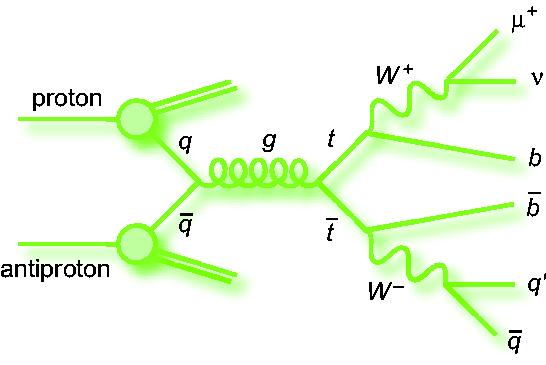
\includegraphics[scale=0.5]{pics_feynman_ttbar_mujets}}
\caption{Feynman-Diagramm eines Top-Antitop-Zerfalls. Im Endzustand sind zwei Quarks, zwei b-Quarks, ein Myon sowie ein Neutrino.}
\label{ttbarsemilep}
\end{figure}

F\"ur die Versuchsdurchf\"uhrung stellen wir Ihnen einen Unix-Rechner und ein Analyse-Framework zur Verf\"ugung. Dieses Framework ist selbstverst\"andlich noch sehr unvollst\"andig und wird w\"ahrend der Versuchsdurchf\"uhrung von Ihnen vervollst\''andigt und erweitert. Kenntnisse in der Programmiersprache C\texttt{++} sind von Vorteil, werden aber nicht vorausgesetzt. Bearbeiten Sie das kurze Tutorial auf
%TODO
\url{https://www.desy.de/~mstoev/teaching/Top_WQS/Cplusplus.pdf}, um sich mit der Syntax in C\texttt{++} vertraut zu machen.\\

